\documentclass [11pt, a4wide, twoside]{article}

\usepackage{times}
%\usepackage{epsfig}
\usepackage{ifthen}
\usepackage{xspace}
\usepackage{fancyhdr}
\usepackage{graphicx}
\usepackage[colorlinks,urlcolor=blue]{hyperref}

% solution switch
\newboolean{showsolution}
\setboolean{showsolution}{true} 
%\setboolean{showsolution}{false}


%layout
\topmargin      -5.0mm
\oddsidemargin  6.0mm
\evensidemargin -6.0mm
\textheight 215.5mm
\textwidth      160.0mm
\parindent        1.0em
\headsep          10.3mm
\headheight        12pt
\lineskip    1pt
\normallineskip     1pt

%header
\lhead{Programming Languages \\ 2021}

\rhead{Prof. O. Nierstrasz\\
Mohammadreza Hazhirpasand, Joel Niklaus}
\lfoot{page \thepage}
\rfoot{\today}
\cfoot{}

\renewcommand{\headrulewidth}{0.1pt}
\renewcommand{\footrulewidth}{0.1pt}

\renewcommand{\thesubsection}{\arabic{subsection}}

%enumeration
\newenvironment{myitemize}{%
     \begin{itemize}
     \setlength{\itemsep}{0cm}}
     {\end{itemize}}

\newenvironment{myenumerate}{%
     \begin{enumerate} \setlength{\itemsep}{0cm}}
     {\end{enumerate}}


%solution
\ifthenelse{\boolean{showsolution}}
   {  \newcommand{\solution}[1]{
   	\noindent\underline{\textbf{Answer:}}\\[2mm]
   	 \textsl{#1}
	 \vspace{10pt}
	 \normalsize
	}
  }
  {  \newcommand{\solution}[1]{} }

\newcounter{exnum}
\def\xexercise{\fontsize{12}{10}\fontseries{bx}\selectfont}
\def\xnormal{\fontseries{m}\fontshape{n}\selectfont}


\newcommand{\exercise}[1]{%
     {\addtocounter{exnum}{1}\vskip 0.8cm{\xexercise \noindent Exercise
\arabic{exnum} (#1)} \xnormal} \vskip 0.3cm} 
 \newcommand{\aufgabe}[1]{
     {\addtocounter{exnum}{1}\vskip 0.8cm{\xexercise \noindent Aufgabe
\arabic{exnum} (#1)} \xnormal} \vskip 0.3cm} 

\pagestyle{fancy}


% ===============ABBREVIATIONS==============================
\newcommand{\eg}{\emph{e.g.,}\xspace}
\newcommand{\ie}{\emph{i.e.,}\xspace}
\newcommand{\etc}{\emph{etc.}\xspace}


\begin{document}

% title
\section*{\ifthenelse{\boolean{showsolution}}{Solution }{}\xspace{}Exam Programming Languages}
\rule{\textwidth}{1pt}\\[1mm]
Date: Friday, 30.05.2013\\
Duration: 70 minutes\\
Material: You are NOT allowed to use any material (e.g., script, exercises including solutions, notes, electronic devices...)\\
Number of exercises: 6\\
Total points: 80 \\
\rule{\textwidth}{1pt}\\[5mm]
Firstname, lastname: \rule{200pt}{0.5pt}\\[5mm]
Matrikel: \rule{200pt}{0.5pt}\\[5mm]
Put your name on each extra page you deliver.\\
Consecutively number all pages. Total number of extra pages: \rule{45pt}{0.5pt}\\
\rule{\textwidth}{1pt}

\newpage
% - - - - - - - - - - - - - - - - - - - - - - - - - - - - - - - - - - - - - - - - - - - - - - - - - - - - - - - - - - - - - - - - - - -

\exercise{20 Points}

\noindent
%
Answer the following questions (do not write more than 3 sentences):

\begin{myenumerate}

%\item Why don't pure functional languages provide loop constructs?	 \textbf{( 2 Points )}
%\solution{Explicit loop constructs are intended to change the state of an entity (object, variable, etc.). But in a pure functional language there is no state because of referential transparency. So itarative processes are accomplished by means of recursion, thus function calls, which does not violate referential transparency.}\vspace{3cm}

\item What is the difference between a static and a dynamic type? Explain and give an example. \textbf{( 4 Points )}
\solution{The static type of a variable or expression is a type which can be determined by the type inference  system solely based on the program code, thus in at compile time. In contrast, the dynamic type of a variable cannot be determined in such a way because the variable may take on different values at runtime. Example:\\
Object x = new Vector();\\
the static type of x is Object, the dynamic type is Vector().}\vspace{2.5cm}

%\item Why is normal order evaluation called lazy? \textbf{( 2 Points )}
%\solution{Because expressions are only evaluated when they are needed, the evaluation is delayed.}\vspace{3cm}

\item Explain how it is possible to use the concept of recursion in the $\lambda$-calculus. \textbf{( 4 Points )}
\solution{We know by the Fixed-Point theorem that every $\lambda$-expression $e$ has a fixed point $p$, i.e. $(e ~p) \equiv p$. Thus recursive functions (i.e. recursive $\lambda$-expressions) can be expressed as fixed-points of other suitable expressions, which must be well-defined. Finding this fixed-point is achieved in the (untyped) lambda-calculus by means of a fixed-point combinator called the \emph{Y-combinator}. So if we define a function $p$ to be the Y-combinator applied to an expression $e$, the result of this application is the again the expression with the desired function as argument, $e~p$, which equals $p$.} \vspace{2.5cm}

\item What is the difference between syntax and semantics? \textbf{( 4 Points )}
\solution{Syntax: the arrangement of words and phrases to create well-formed sentences in a language \\
Semantics: the meaning of a word, phrase, sentence or text\\
You can create well-formed sentences (according to the syntax) that don't have a meaning (according to semantics).} \vspace{2.5cm}

%\newpage
%\item How does contravariance support subtyping?\textbf{( 2 Points )}
%\solution{Because the contravariance parameter type will always end in the correct result subclass since $f_y$ is a superset of $f_x$} \vspace{3cm}

% JavaScript (2 questions)
\item Can you implement prototype inheritance in Java using delegation? Explain. \textbf{( 4 Points )}
\solution{No, Java's delegation do not support this to be bounded to the delegating object. Unless one use explicit argument.} \vspace{2.5cm}

\item What is the difference between this in Java and Javascript? Consider from the point of view of delegation. \textbf{( 4 Points )}
\solution{Java does not support this to be bounded to the delegating object. In Javascript, this is bounded to the delegating object.} \vspace{2.5cm}

\item How do you extend all objects created with a specific constructor?  \textbf{( 2 Points )}
\solution{if the constructor is \texttt{Counter} then \texttt{Counter.prototype} -- very easy question!}
%\item What happen if we assign a variable without using the command ``var''? What problem can it cause? \textbf{( 2 Points )}
%\solution{We override the variable in the closest scope in a scope chain. If no such variable exists, the global variable is created.} \vspace{3cm}

\item Where do you define properties that are shared between a group of objects, e.g. static variables. \textbf{( 2 Points )}
\solution{if the constructor of the objects is Counter, than Counter.value is a shared between all the instances}

% Prolog (2 questions)
\item Is there a difference between logical negation \texttt{$\neg$} and \texttt{not} operator implemented using cut and fail? Explain. \textbf{( 4 Points )} \\
\texttt{not(X) :- X!, fail. } \\
\texttt{not(\_).}
\solution{Yes, cut and fail $A \wedge \neg B = \neg B \wedge A$ but $A, not(B) \not = not(B), A$} \vspace{2.5cm}

\item In which cases does Prolog assume that the answer to a query is false? \textbf{( 2 Points )}
\solution{Close world assumption. If cannot infer true, then false}

\item What is a Horn Clause? What is Head and Body? \textbf{( 2 Points )}
\solution{A if A1 and A2 and A3 ... and AN.  A is Head, A1 and A2 ... and AN is a body.}
\end{myenumerate}


\newpage
% - - - - - - - - - - - - - - - - - - - - - - - - - - - - - - - - - - - - - - - - - - - - - - - - - - - - - - - - - - - - - - - - - - -

\exercise{5 Points}
\noindent
%

A very junior programmer wanted to write the ``hello world'' program in post script. Here is the result: 

\begin{small}
\begin{verbatim}
/Times-Roman findfont
    18 scalefont
    setfont
100 500 moveto

/myprint {
    /mystring exch def
    mystring show
} def

/mystring (World) def
(Hello) myprint
mystring myprint
showpage
\end{verbatim}
\end{small}

\begin{myenumerate}
\item Did the programmer succeed? What is the output and why?
\end{myenumerate}

\solution{The result is HelloHello since the first call to my print will redefine /mystring.}



\newpage
% - - - - - - - - - - - - - - - - - - - - - - - - - - - - - - - - - - - - - - - - - - - - - - - - - - - - - - - - - - - - - - - - - - -

\exercise{20 Points}
\noindent
%
\begin{enumerate}
\item Write a Haskell program that, given a number, determines if the number is a Fibonacci Number or not. If it is return true, else false. Write down the types of the functions you write.
\vspace{9cm}
\solution { 
sources/haskell.hs
}
\item If we list all the natural numbers below 10 that are multiples of 3, we get 3, 6 and 9. The sum of these multiples is 18.

Write a Haskell program that finds the sum of all the multiples of 3 below 1000. Write down the types of the functions you write.
\vspace{6cm}
\solution { 
sources/haskell.hs
}
\end{enumerate}



\newpage
% - - - - - - - - - - - - - - - - - - - - - - - - - - - - - - - - - - - - - - - - - - - - - - - - - - - - - - - - - - - - - - - - - - -

\exercise{15 Points}
\noindent
%
\begin{enumerate}
\item Consider the following $\lambda$-expressions. Indicate which occurrences of
variables are bound and which ones are free in the expressions.
\begin{enumerate}
\item \texttt{($\lambda$ a b .~c d a b) a b ($\lambda$ c d .~d c)($\lambda$ e f .~f) e} \vspace{1cm}

\item \texttt{(($\lambda$ u v .~$\lambda$ w .~w ($\lambda$ x .~x(u)) (v)) (y)) ($\lambda$ z .~$\lambda$ y .~z(y))}\vspace{1cm}

\item \texttt{$\lambda$ y .~($\lambda$ x .~z(x($\lambda$ x .~y(z)))) ($\lambda$ z .~y(x(z)))}\vspace{1cm}
\end{enumerate}

\solution{\fontsize{9pt}{11pt}\texttt{($\lambda$ a b .~c a b) a b ($\lambda$ c d .~d c)($\lambda$ e f .~f) }\\
\texttt{($\lambda$ a b .~f b b) f f ($\lambda$ c d .~b b)($\lambda$ e f .~b) }\\

\noindent
\texttt{(($\lambda$ u v .~$\lambda$ w .~w ($\lambda$ x .~x(u)) (v)) (y)) ($\lambda$ z .~$\lambda$ y .~z(y))}\\
\texttt{(($\lambda$ u v .~$\lambda$ w .~b ($\lambda$ x .~b(b)) (b)) (f)) ($\lambda$ z .~$\lambda$ y .~b(b))}\\

\noindent
\texttt{($\lambda$ y .~$\lambda$ x .~z(x($\lambda$ x .~y(z)))) ($\lambda$ z .~y(x(z)))}\\
\texttt{($\lambda$ y .~$\lambda$ x .~f(b($\lambda$ x .~b(f)))) ($\lambda$ z .~f(f(b)))}\\\\

\noindent
\texttt{($\lambda$ x y .~y x) ($\lambda$ x y .~y x)($\lambda$ x .~x x)($\lambda$ y .~y)} \\
\texttt{($\lambda$ x .~x x)($\lambda$ x y .~y x)($\lambda$ y .~y)} \\
\texttt{($\lambda$ x y .~y x)($\lambda$ x y .~y x)($\lambda$ y .~y)}\\ 
\texttt{($\lambda$ y .~y)($\lambda$ x y .~y x)} \\
\texttt{($\lambda$ x y .~y x)} \\}

\item Reduce the following $\lambda$-expressions to their normal form.
\begin{enumerate}
\item \texttt{((($\lambda$ Q . ($\lambda$ x . (Q x))) P) j)} \vspace{4cm}

\solution{(P j)}

\item \texttt{(((($\lambda$ G . ($\lambda$ L.($\lambda$ x.((G L) x)))) A) P) j)}\vspace{4cm}

\solution{((A P) j)}

\item \texttt{(($\lambda$ x . (($\lambda$ x . (K x x)) j)) m)}\vspace{4cm}
\solution{(K j j)}
\end{enumerate}
\end{enumerate}




\newpage
% - - - - - - - - - - - - - - - - - - - - - - - - - - - - - - - - - - - - - - - - - - - - - - - - - - - - - - - - - - - - - - - - - - -


\newpage
% - - - - - - - - - - - - - - - - - - - - - - - - - - - - - - - - - - - - - - - - - - - - - - - - - - - - - - - - - - - - - - - - - - -
% Javascript
\exercise{10 Points}

\noindent Suppose you have a small JavaScript program with a database of people:
\begin{verbatim}
var alice = Object.create(person);
alice.name = "Alice";
alice.age = 22;

var bob = Object.create(person);
bob.name = "Bob";
bob.age = 29;

var cyril = Object.create(person);
cyril.name = "Bob";
cyril.age = 45;
\end{verbatim}


\begin{enumerate}
        \item What is the parent of Alice, Bob and Cyril? \textbf{(~1~Points~)}
        \vspace{5cm}
        \solution{\texttt{Person}}

        \item You realize, you need to change the parent of Alice and Bob to \texttt{Employee}, the Cyril to \texttt{Manager}. How would you do it? \textbf{(~2~Points~)}
        \vspace{5cm}
        \solution{\begin{verbatim}
var employee = Object.create(person);
var manager = Object.create(person);

alice.__proto__ = employee.
bob.__proto__ = employee.
cyril.__proto__ = manager.
\end{verbatim}
}

        \item A manager has to be responsible. How would make Cyril (only Cyril) to respond to the message \texttt{isResponsible}? \textbf{(~2~Points~)}
        \vspace{5cm}
        \solution{\begin{verbatim}
manager.isResponsible = function() {
    alert("I am very responsible");
}
\end{verbatim}
}

        \item Bob wants to be manager as well, so he tries to be responsible as well. How would you make Bob to become responsible? \textbf{( 2 Points )}
        \vspace{5cm}
        \solution{\begin{verbatim}
bob.isResponsible = manager.isResponsible.
\end{verbatim}
}
\end{enumerate}



\newpage
\exercise{10 Points}
A possible classification for cars is the one shown in Figure. 
When it comes to classify the Hybrid Cars (Type C) you realize that it tanks gas and it also charges. 
So implement the class diagram shown in the figure including the Type C hybrid car in JavaScript. 
Do not copy-paste any code!

\begin{figure}[h!]
  \centering{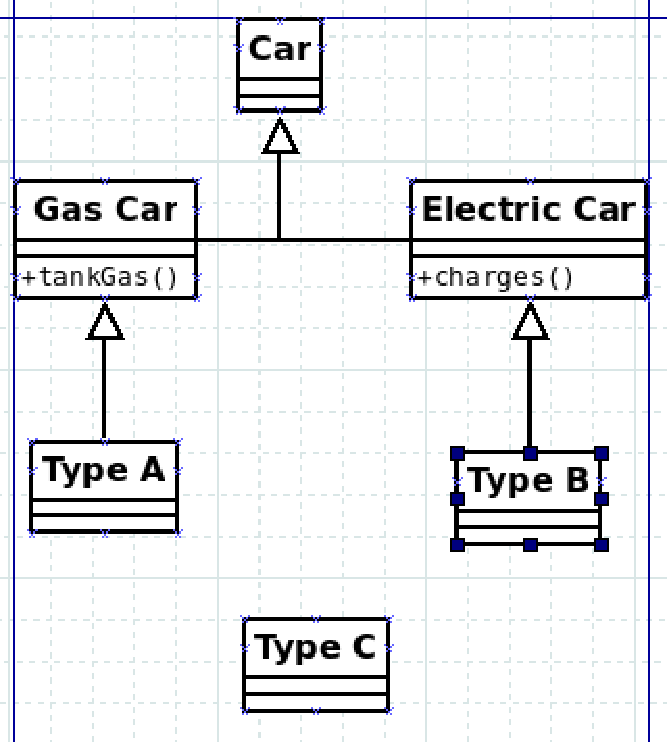
\includegraphics[width=1\columnwidth]{images/cars}}\caption{Possible classification of cars.}\label{cars}
\end{figure}

\solution{\begin{verbatim}
var car = {}

var gasCar = Object.create(car);
gasCar.tankGas = function () {
	alert("I tank gas!");
}

electricCar = Object.create(car);
dolphin.charges = function() {
	alert("I can charge myself");
}

var typeA = Object.create(gasCar);

var typeB = Object.create(electricCAr);


var typeC = Object.create(gasCar);
typeC.charges = electricCar.charges;
\end{verbatim}

}

% - - - - - - - - - - - - - - - - - - - - - - - - - - - - - - - - - - - - - - - - - - - - - - - - - - - - - - - - - - - - - - - - - - -
%Prolog
\newpage
\exercise{10 Points}
How would you write a program in Prolog that solves the hanoi tower problem?

\noindent Define a predicate \texttt{hanoi(N, A, B, C, Moves)} that solves the hanoi-towers problem. 
\texttt{Moves} holds the list of moves that represent the process of moving \texttt{N} disks from \texttt{A} to \texttt{B} with the help of \texttt{C}. 
If \texttt{N} is bigger than 1, then \texttt{N-1} disks will be shifted to \texttt{C}, so that the move from \texttt{A} to \texttt{B} can be accomplished. 
The move of a disk from \texttt{A} to \texttt{B} will be represented as \texttt{[a to b]}. 
The binary operator \emph{to} is loaded into the knowledge base by the following commands:
\begin{verbatim}
  :- ensure_loaded(library(operators)). % load readable operators
  :- op(900, xfy, to).                  % define new infix operator 'to'
\end{verbatim}
\noindent Examples:
\begin{verbatim}
  ?- hanoi(1,a,b,c,X).		
  X = [a to b] ?			
  yes					

  ?- hanoi(2,a,b,c,X).
  X = [a to c, a to b, c to b] ?
  yes
\end{verbatim}


\solution{\begin{verbatim}
%ensure_loaded(library(operators)).
%op(900, xfy, to).

hanoi(1,A,B,_,[A to B]). 
hanoi(N,A,B,C,S) :- 
	N > 1,
	N1 is N - 1,
	hanoi(N1, A,C,B, S1),
	append(S1, [A to B], S2),
	hanoi(N1, C,B,A, S3),
	append(S2, S3, S).
\end{verbatim}
}

\newpage
\exercise{10 Points}

\begin{figure}[h!]
  \centering{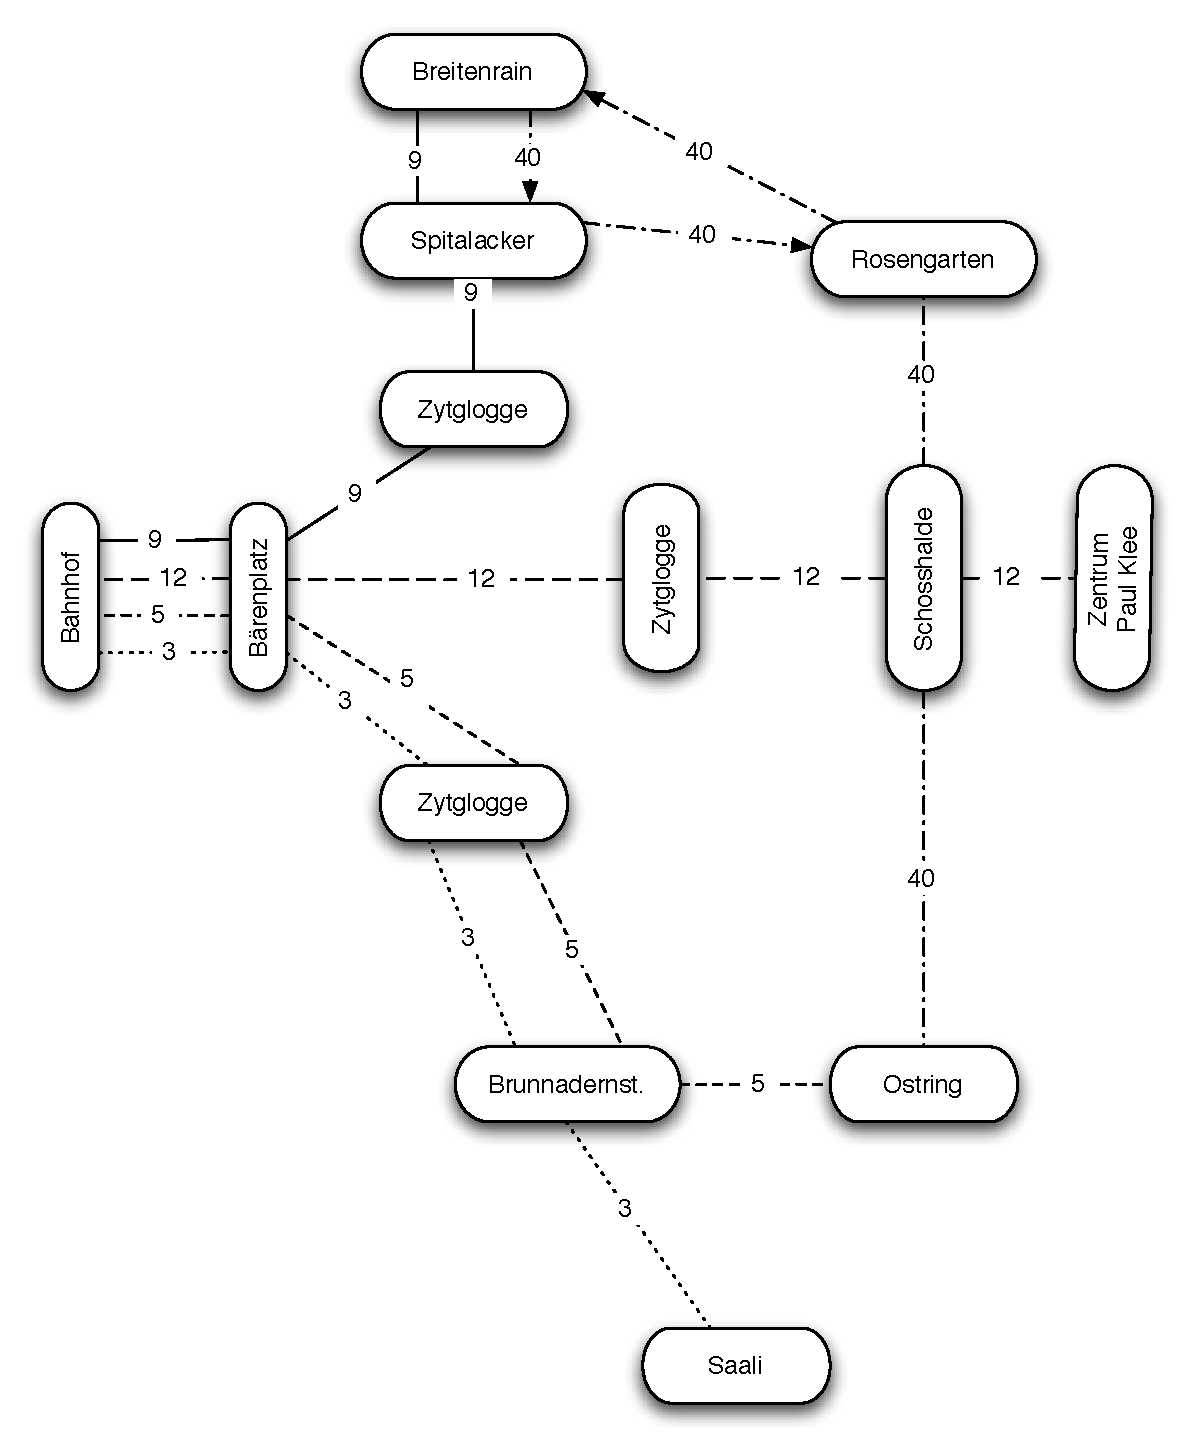
\includegraphics[width=0.6\columnwidth]{images/tram}}\caption{Simplified public transport network of Berne.}\label{tram}
\end{figure}

\noindent
The tram and bus lines shown in Fig., \ref{tram} are represented by the following database of connections:

\begin{small}
\begin{verbatim}
connected(breitenrain,spitalacker,9). 
connected(breitenrain,spitalacker,40). 
connected(spitalacker,rosengarten,40). 
connected(spitalacker,breitenrain,9). 
connected(spitalacker,zytglogge,9). 
connected(zytglogge,baerenplatz,9). 
connected(zytglogge,baerenplatz,12). 
connected(zytglogge,baerenplatz,3). 
connected(zytglogge,baerenplatz,5). 
connected(zytglogge,spitalacker,9). 
connected(zytglogge,schosshalde,12). 
connected(zytglogge,brunnadernst,3). 
connected(zytglogge,brunnadernst,5). 
connected(baerenplatz,bahnhof,3). 
connected(baerenplatz,bahnhof,5). 
connected(baerenplatz,bahnhof,9). 
connected(baerenplatz,bahnhof,12). 
connected(bahnhof,baerenplatz,3). 
connected(bahnhof,baerenplatz,5). 
connected(bahnhof,baerenplatz,9). 
connected(bahnhof,baerenplatz,12). 
connected(brunnadernst,zytglogge,3). 
connected(brunnadernst,zytglogge,5). 
connected(brunnadernst,ostring,5). 
connected(brunnadernst,saali,3). 
connected(saali,brunnadernst,3). 
connected(ostring,brunnadernst,5). 
connected(ostring,schosshalde,40). 
connected(schosshalde,zytglogge,12). 
connected(schosshalde,rosengarten,40). 
connected(schosshalde,zentrumpaulklee,12). 
connected(schosshalde,ostring,40). 
connected(zentrumpaulklee,schosshalde,12). 
connected(rosengarten,schosshalde,40). 
connected(rosengarten,breitenrain,40).
\end{verbatim}
\end{small}


\begin{enumerate}
\item Define a prolog predicate \texttt{reachable/2} which is true if you can reach the second station from the first by using one or more lines (line numbers do not matter). \textbf{( 5 points )} \vspace{5cm}
\item Define another prolog predicate \texttt{reachableBy/3} which is true if an arbitrary station is reachable from another station by a given, single line number. \textbf{( 5 points )}\vspace{5cm}
\end{enumerate}



\solution{\fontsize{8}{10}\begin{verbatim}
% b)

reachable(X,Y) :- reachableVia(X,Y,[X]). 
reachableVia(X,Y,S) :- connected(X,Y,_), not(in(Y,S)). 
reachableVia(X,Y,S) :- connected(X,A,_), not(in(A,S)), reachableVia(A,Y,[A|S]).

% c)
	
reachableBy(X,Y,Z) :- reachableByVia(X,Y,Z,[X]). 
reachableByVia(X,Y,Z,S) :- connected(X,Y,Z), not(in(Y,S)). 
reachableByVia(X,Y,Z,S) :- connected(X,A,Z), not(in(A,S)), reachableByVia(A,Y,Z,[A|S]). 

% helper
in(X,[X|_]).
in(X,[_|L]):- in(X,L).
not(X):- (X -> fail); true.
\end{verbatim}}


\exercise{10 Points}
% - - - - - - - - - - - - - - - - - - - - - - - - - - - - - - - - - - - - - - - - - - - - - - - - - - - - - - - - - - - - - - - - - - -
Consider the following directed graph:

\begin{figure}[h]
\centering{\fbox{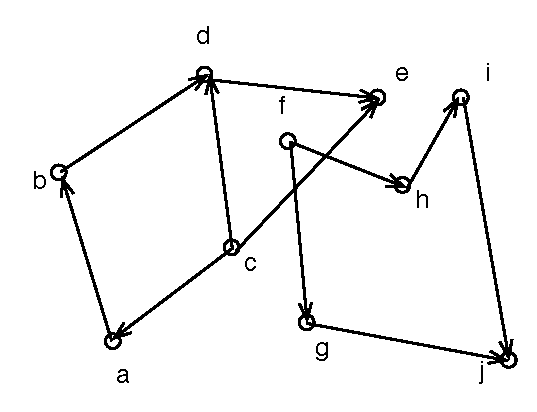
\includegraphics[width=6cm]{images/map.pdf}}}
\end{figure}

Write a Prolog database consisting of the following predicates:

\begin{enumerate}
\renewcommand{\theenumi}{\alph{enumi}}

\item \texttt{line(p1,p2)} that is true iff there is a direct connection between \texttt{p1} and \texttt{p2}.

\item \texttt{triangle(p1,p2,p3)} that is true iff \texttt{p1}, \texttt{p2}, and \texttt{p3} form a triangle (independent of the connection directions).

\item \texttt{quadrangle(p1,p2,p3,p4)} that is true iff \texttt{p1}, \texttt{p2}, \texttt{p3}, and \texttt{p4} form a quadrangle (independent of the connection directions).

\item \texttt{reachable(p1,p2)} that is true iff there is a directed path from \texttt{p1} to \texttt{p2} (i.e. iff \texttt{p2} is reachable from \texttt{p1} respecting the connection directions).
\end{enumerate}

\solution{\begin{verbatim}
connection(A,B) :- line(A,B); line(B,A).
in(X,[X|_]).
in(X,[_|L]):- in(X,L).

line(a,b).
line(b,d).
line(c,a).
line(c,d).
line(c,e).
line(d,e).
line(f,g).
line(f,h).
line(g,j).
line(h,i).
line(i,j).


triangle(A,B,C) :- connection(A,B), connection(B,C), connection(C,A).


quadrangle(A,B,C,D) :- connection(A,B), connection(B,C), connection(C,D), connection(D,A), 
                       not(in(D,[A,B,C])).

reachable(X,Y) :- line(X,Y).
reachable(X,Y) :- line(X,Z), reachable(Z,Y).
\end{verbatim}
}

% - - - - - - - - - - - - - - - - - - - - - - - - - - - - - - - - - - - - - - - - - - - - - - - - - - - - - - - - - - - - - - - - - - -

% - - - - - - - - - - - - - - - - - - - - - - - - - - - - - - - - - - - - - - - - - - - - - - - - - - - - - - - - - - - - - - - - - - -
\newpage
\subsection*{Points}

\begin{minipage}[t]{120pt}
\textbf{Exercise 1}
\vspace{5pt}\\
\begin{tabular}{|c|c|c|c|}
\hline
Task & Points & Score \\\hline
1 & 4 & \\\hline
2 & 4 & \\\hline
3 & 4 & \\\hline
4 & 4 & \\\hline
5 & 4 & \\\hline
\textbf{Total} & \textbf{20} &\\\hline\hline
\end{tabular}
\end{minipage}
\begin{minipage}[t]{120pt}


\textbf{Exercise 2}
\vspace{5pt}\\
\begin{tabular}{|c|c|c|c|}
\hline
Task & Points & Score \\\hline
1 & 5 & \\\hline
\textbf{Total} & \textbf{5} &\\\hline\hline
\end{tabular}
\end{minipage}
\begin{minipage}[t]{120pt}


\textbf{Exercise 3}
\vspace{5pt}\\
\begin{tabular}{|c|c|c|c|}
\hline
Task & Points & Score \\\hline
1 & 10 & \\\hline
2 & 10 & \\\hline
\textbf{Total} & \textbf{20} &\\\hline\hline
\end{tabular}
\end{minipage}
\begin{minipage}[t]{120pt}


\textbf{Exercise 4}
\vspace{5pt}\\
\begin{tabular}{|c|c|c|c|}
\hline
Task & Points & Score \\\hline
1 & 5 & \\\hline
2 & 10 & \\\hline
\textbf{Total} & \textbf{15} &\\\hline\hline
\end{tabular}
\end{minipage}

\noindent
\begin{minipage}[t]{120pt}

\vspace{1cm}

\textbf{Exercise 5}
\vspace{5pt}\\
\begin{tabular}{|c|c|c|c|}
\hline
Task & Points & Score \\\hline
1 & 2 & \\\hline
1 & 2 & \\\hline
1 & 4 & \\\hline
1 & 2 & \\\hline
\textbf{Total} & \textbf{10} &\\\hline\hline
\end{tabular}
\end{minipage}
\begin{minipage}[t]{120pt}
\vspace{1cm}

\textbf{Exercise 6}
\vspace{5pt}\\
\begin{tabular}{|c|c|c|c|}
\hline
Task & Points & Score \\\hline
1 & 5 & \\\hline
2 & 5 & \\\hline
\textbf{Total} & \textbf{10} &\\\hline\hline
\end{tabular}
\vspace{5cm}

\textbf{TOTAL}
\vspace{5pt}\\
\begin{tabular}{|c|c|c|c|}
\hline
Task & Points & Score \\\hline
1 & 20 & \\\hline
2 & 5 & \\\hline
3 & 20 & \\\hline
4 & 15 & \\\hline
10 & 10 & \\\hline
6 & 10 & \\\hline
\textbf{Total} & \textbf{80} &\\\hline\hline
\end{tabular}
\end{minipage}

\end{document}
